\documentclass[tikz]{standalone}
\usetikzlibrary {automata,positioning,fit,calc} 
\usetikzlibrary{decorations.pathreplacing,calligraphy}
\usepackage{inconsolata}
\begin{document}
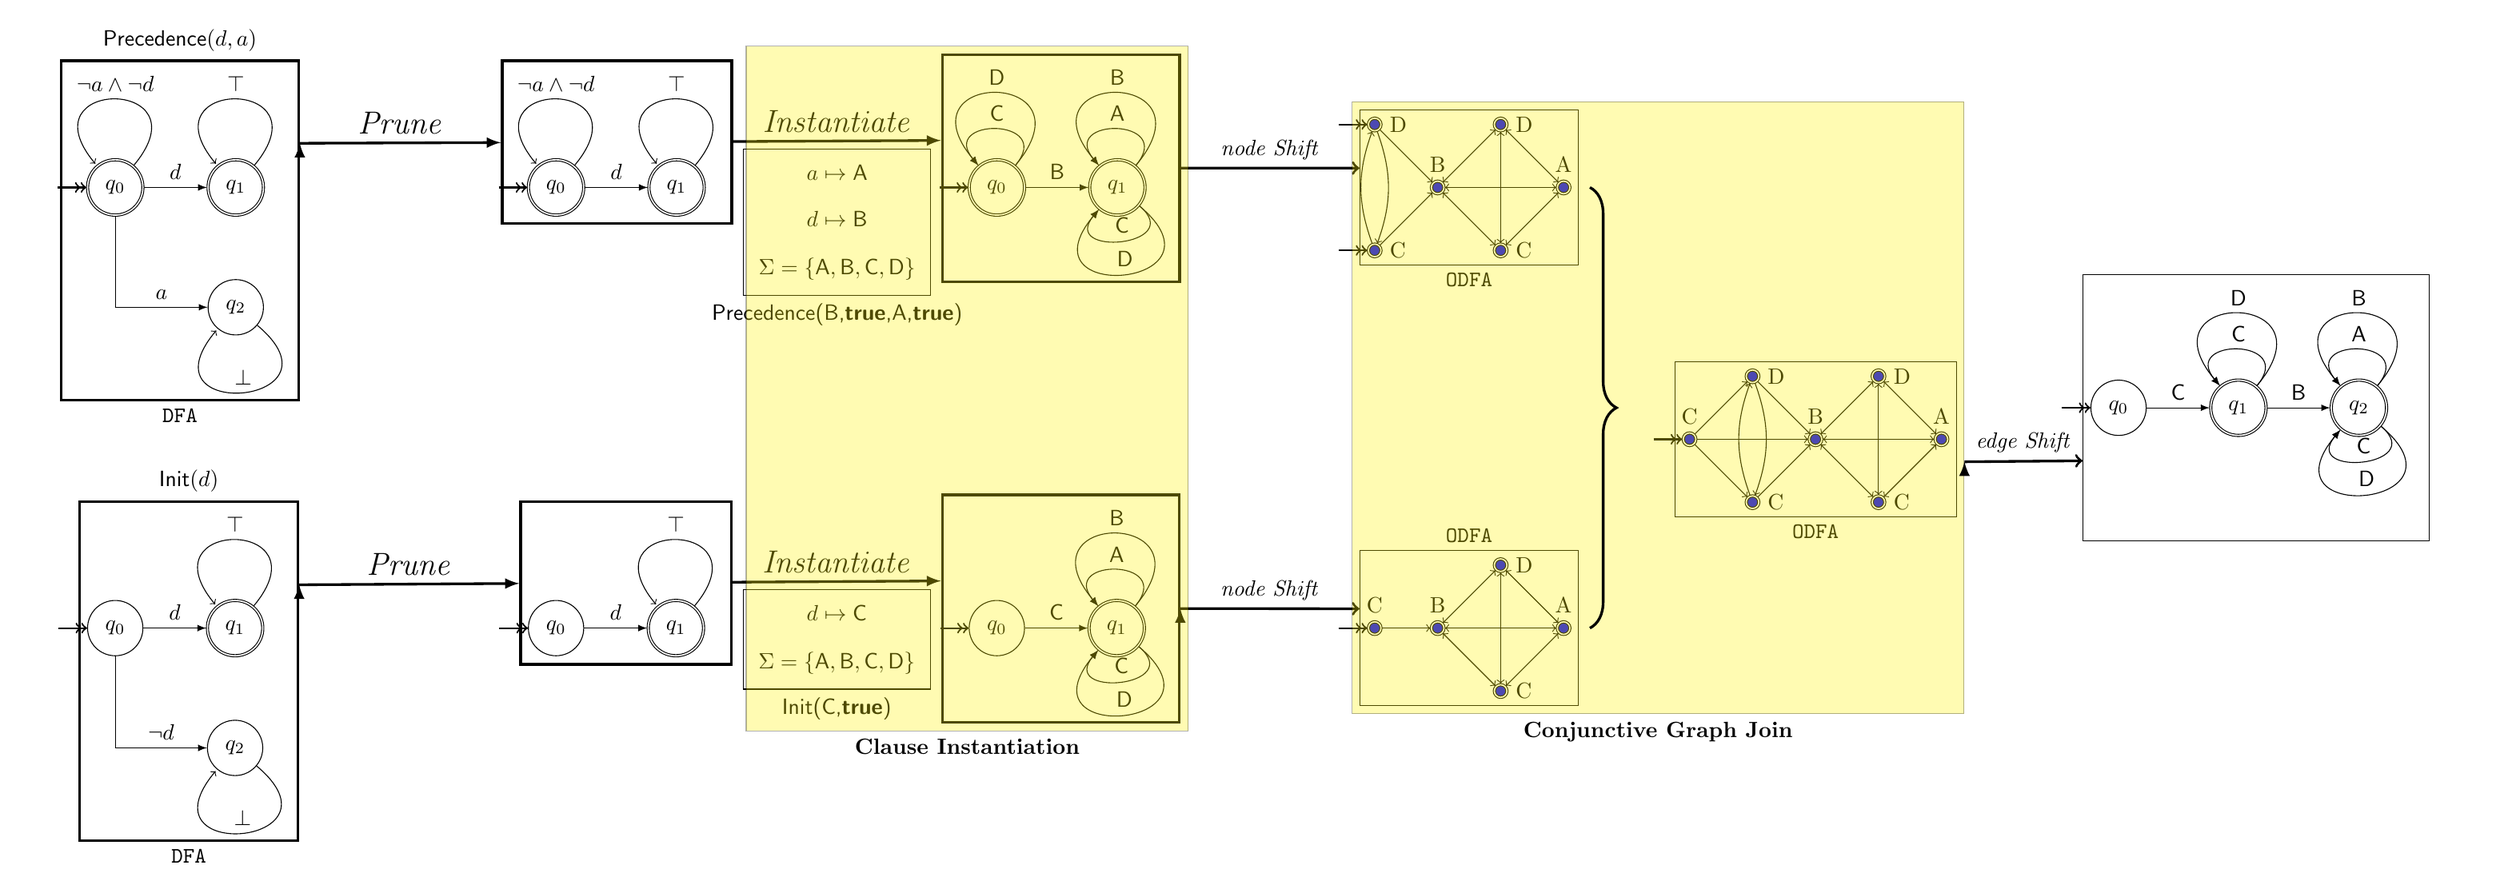
\begin{tikzpicture}[every initial by arrow/.style={text={},->>,thick},-latex,initial text={}]


%%%%%%%%%%%%%%%%%%%%%% PRECEDENCE

\node[state,accepting,initial] (q0) {$q_0$};
\draw[-latex] (q0) edge[in=130,out=50,loop,-latex] node[above] (e1) {$\neg a\wedge \neg d$} ();%
\node[state,accepting,right=of q0] (q1) {$q_1$};
\node[state,below=of q1] (q2) {$q_2$};
\draw[-latex] (q0) |- (q2) node[near end,above] {$a$};
\draw[-latex] (q0) edge node[above] {$d$} (q1);
\draw[-latex] (q1) edge[in=130,out=50,loop] node[above] {$\top$} ();%
\draw[-latex] (q2) edge[in=230,out=320,loop] node[above] (e2){$\bot$} ();%
\coordinate (P) at ($(e2.south east)+(.5,0)$) ;

\node[draw,fit=(q0)(q1)(q2)(e1)(P),very thick,label=south:{\texttt{DFA}},label=north:{\textsf
{Precedence}($d,a$)}] (B1A) {};


\node[state,accepting,initial] at (7,0) (q02) {$q_0$};
\draw[-latex] (q02) edge[in=130,out=50,loop,-latex] node[above] (e3) {$\neg a\wedge \neg d$} ();%
\node[state,accepting,right=of q02] (q12) {$q_1$};
\draw[-latex] (q02) edge node[above] {$d$} (q12);
\draw[-latex] (q12) edge[in=130,out=50,loop] node[above] (e5) {$\top$} ();%

\node[state,accepting,initial] at (14,0) (q03) {$q_0$};
\path[-latex,draw] (q03) to  [in=130,out=50,loop,-latex,distance=1cm] node[above] {$\textsf{C}$} (q03);
\path[-latex,draw] (q03) to  [in=130,out=50,loop,-latex,distance=2cm] node[above] (e1) {$\textsf{D}$} (q03);
\coordinate (P5) at ($(e5.north east)+(.5,0)$) ;

\node[draw,fit=(q02)(q12)(e3.north west)(P5),very thick] (B2A) {};
        
\node[state,accepting,right=of q03] (q13) {$q_1$};
\draw[-latex] (q03) edge node[above] {$\textsf{B}$} (q13);
\path[-latex,draw] (q13) to  [in=130,out=50,loop,-latex,distance=1cm] node[above] {$\textsf{A}$} (q13);
\path[-latex,draw] (q13) to  [in=130,out=50,loop,-latex,distance=2cm] node[above](e2) {$\textsf{B}$} (q13);

\path[-latex,draw] (q13) to  [in=230,out=320,loop,-latex,distance=1cm] node[above] {$\textsf{C}$} (q13);
\path[-latex,draw] (q13) to  [in=230,out=320,loop,-latex,distance=2cm] node[above] (e4) {$\textsf{D}$} (q13);
\coordinate (P4) at ($(e4.south east)+(.5,0)$) ;
\coordinate (P2) at ($(e1.south east)-(1,0)$) ;
\node[draw,fit=(q03)(q13)(e1)(P2)(P4),very thick] (B3A) {};



\draw[very thick] (B1A.36) edge[-latex] node[midway,above] {\Large\textit{Prune}} (B2A);
\draw[-latex,very thick] (B2A) edge node[above] (j2) {\Large\textit{Instantiate}} (B3A.167) ;%

\node[below=.25cm of j2] (tn1) {$a\mapsto\textsf{A}$};
\node[below=.25cm of tn1] (tn2) {$d\mapsto\textsf{B}$};
\node[below=.25cm of tn2] (tn3) {$\Sigma=\{\textsf{A},\textsf{B},\textsf{C},\textsf{D}\}$};
\node[draw,fit=(tn1)(tn2)(tn3),label=south:{\textsf{Precedence(\textsf{B},\textbf{true},\textsf{A},\textbf{true})}}] (tn) {};


\node[draw,circle,minimum size=2mm,inner sep=0pt,outer sep=0pt,fill=blue,label=east:{D},initial,accepting] at (20,1) (da) {};
\node[draw,circle,minimum size=2mm,inner sep=0pt,outer sep=0pt,fill=blue,label=east:{C},initial,accepting] at (20,-1) (ca) {};
\node[draw,circle,minimum size=2mm,inner sep=0pt,outer sep=0pt,fill=blue,label=north:{B},accepting] at (21,0) (bb) {};
\node[draw,circle,minimum size=2mm,inner sep=0pt,outer sep=0pt,fill=blue,label=east:{D},accepting] at (22,1) (db) {};
\node[draw,circle,minimum size=2mm,inner sep=0pt,outer sep=0pt,fill=blue,label=east:{C},accepting] at (22,-1) (cb) {};
\node[draw,circle,minimum size=2mm,inner sep=0pt,outer sep=0pt,fill=blue,label=north:{A},accepting] at (23,0) (ab) {};

  \path[->]          (da)  edge   [bend left=20]   (ca);
  \path[->]          (ca)  edge   [bend left=20]   (da);
\draw[->] (da) -- (bb);
\draw[->] (ca) -- (bb);
\draw[<->] (db) -- (cb);
\draw[<->] (db) -- (bb);
\draw[<->] (cb) -- (bb);
\draw[<->] (db) -- (ab);
\draw[<->] (cb) -- (ab);
\draw[<->] (bb) -- (ab);
\node[draw,fit=(da.north)(ca)(db)(cb)(ab),label=south:{\texttt{ODFA}}] (op1) {};
\draw[very thick] (B3A) edge[->] node[above] {\textit{node Shift}} (op1.170);
%%%%%%%%%%%%%%%%%%%%%%%%%%%%% Init

\node[state,initial] at (0,-7) (q0) {$q_0$};
\node[state,accepting,right=of q0] (q1) {$q_1$};
\node[state,below=of q1] (q2) {$q_2$};
\draw[-latex] (q0) |- (q2) node[near end,above] {$\neg d$};
\draw[-latex] (q0) edge node[above] {$d$} (q1);
\draw[-latex] (q1) edge[in=130,out=50,loop] node[above] (ten) {$\top$} ();%
\draw[-latex] (q2) edge[in=230,out=320,loop] node[above] (e2){$\bot$} ();%
\coordinate (P) at ($(e2.south east)+(.5,0)$) ;

\node[draw,fit=(q0)(q1)(q2)(ten)(P),very thick,label=south:{\texttt{DFA}},label=north:{\textsf
{Init}($d$)}] (B1) {};



\node[state,initial] at (7,-7) (q02) {$q_0$};
\node[state,accepting,right=of q02] (q12) {$q_1$};
\draw[-latex] (q02) edge node[above] {$d$} (q12);
\draw[-latex] (q12) edge[in=130,out=50,loop] node[above] (e5) {$\top$} ();%

\node[state,initial] at (14,-7) (q03) {$q_0$};
\coordinate (P5) at ($(e5.north east)+(.5,0)$) ;
\node[draw,fit=(q02)(q12)(P5),very thick] (B2) {};
        
\node[state,accepting,right=of q03] (q13) {$q_1$};
\draw[-latex] (q03) edge node[above] {$\textsf{C}$} (q13);
\path[-latex,draw] (q13) to  [in=130,out=50,loop,-latex,distance=1cm] node[above] {$\textsf{A}$} (q13);
\path[-latex,draw] (q13) to  [in=130,out=50,loop,-latex,distance=2cm] node[above](e2) {$\textsf{B}$} (q13);

\path[-latex,draw] (q13) to  [in=230,out=320,loop,-latex,distance=1cm] node[above] {$\textsf{C}$} (q13);
\path[-latex,draw] (q13) to  [in=230,out=320,loop,-latex,distance=2cm] node[above] (e4) {$\textsf{D}$} (q13);
\coordinate (P47) at ($(e4.south east)+(.5,0)$) ;
\coordinate (P27) at ($(e1.south east)-(1,6.5)$) ;
\node[draw,fit=(P27)(P47),very thick] (B3) {};



\draw[very thick] (B1.38) edge[-latex] node[midway,above] {\Large\textit{Prune}} (B2);
\draw[-latex,very thick] (B2) edge node[above] (j) {\Large\textit{Instantiate}} (B3.167) ;%

\node[below=.25cm of j] (tn2) {$d\mapsto\textsf{C}$};
\node[below=.25cm of tn2] (tn3) {$\Sigma=\{\textsf{A},\textsf{B},\textsf{C},\textsf{D}\}$};
\node[draw,fit=(tn2)(tn3),label=south:{\textsf{Init(\textsf{C},\textbf{true})}}] (tn2) {};


\node[draw,circle,minimum size=2mm,inner sep=0pt,outer sep=0pt,fill=blue,label=north:{C},initial,accepting] at (20,-7) (cab) {};
\node[draw,circle,minimum size=2mm,inner sep=0pt,outer sep=0pt,fill=blue,label=north:{B},accepting] at (21,-7) (bbb) {};
\node[draw,circle,minimum size=2mm,inner sep=0pt,outer sep=0pt,fill=blue,label=east:{D},accepting] at (22,-6) (dbb) {};
\node[draw,circle,minimum size=2mm,inner sep=0pt,outer sep=0pt,fill=blue,label=east:{C},accepting] at (22,-8) (cbb) {};
\node[draw,circle,minimum size=2mm,inner sep=0pt,outer sep=0pt,fill=blue,label=north:{A},accepting] at (23,-7) (abb) {};

\draw[->] (cab) -- (bbb);
\draw[<->] (dbb) -- (cbb);
\draw[<->] (dbb) -- (bbb);
\draw[<->] (cbb) -- (bbb);
\draw[<->] (dbb) -- (abb);
\draw[<->] (cbb) -- (abb);
\draw[<->] (bbb) -- (abb);

\node[draw,fit=(cab)(dbb)(cbb)(abb),label=north:{\texttt{ODFA}}] (op2) {};
\draw[very thick] (B3.0) edge[->] node[above] {\textit{node Shift}} (op2.170);

\node[draw,circle,minimum size=2mm,inner sep=0pt,outer sep=0pt,fill=blue,label=north:{C},initial,accepting] at (25,-4) (car) {};
\node[draw,circle,minimum size=2mm,inner sep=0pt,outer sep=0pt,fill=blue,label=east:{D},accepting] at (26,-3) (da2r) {};
\node[draw,circle,minimum size=2mm,inner sep=0pt,outer sep=0pt,fill=blue,label=east:{C},accepting] at (26,-5) (ca2r) {};
\node[draw,circle,minimum size=2mm,inner sep=0pt,outer sep=0pt,fill=blue,label=north:{B},accepting] at (27,-4) (bbr) {};
\node[draw,circle,minimum size=2mm,inner sep=0pt,outer sep=0pt,fill=blue,label=east:{D},accepting] at (28,-3) (dbr) {};
\node[draw,circle,minimum size=2mm,inner sep=0pt,outer sep=0pt,fill=blue,label=east:{C},accepting] at (28,-5) (cbr) {};
\node[draw,circle,minimum size=2mm,inner sep=0pt,outer sep=0pt,fill=blue,label=north:{A},accepting] at (29,-4) (abr) {};

\draw[->] (car) -- (bbr);
\draw[->] (car) -- (ca2r);
\draw[->] (car) -- (da2r);
\draw[<->] (dbr) -- (cbr);
\draw[<->] (dbr) -- (bbr);
\draw[<->] (cbr) -- (bbr);
\draw[<->] (dbr) -- (abr);
\draw[<->] (cbr) -- (abr);
\draw[<->] (bbr) -- (abr);
  \path[->]          (da2r)  edge   [bend left=20]   (ca2r);
  \path[->]          (ca2r)  edge   [bend left=20]   (da2r);\draw[->] (da2r) -- (bbr);
\draw[->] (ca2r) -- (bbr);

\node[draw,fit=(car)(dbr)(cbr)(abr),label=south:{\texttt{ODFA}}] (op3) {};
\node[draw,fit=(op1)(op2)(op3),label=south:{\textbf{Conjunctive Graph Join}},fill=yellow,opacity=.3] (cgj) {};
\node[draw,fit=(j)(B3A)(j2)(B3),label=south:{\textbf{Clause Instantiation}},fill=yellow,opacity=.3] {};
\draw [decorate,
    decoration = {brace,raise=5pt,amplitude=12pt},very thick,-] (op1.east) --  (op2.east);



\node[state,initial,right=2cm of cgj] (q03A) {$q_0$};
\node[state,accepting,right=of q03A] (q03V) {$q_1$};
\draw[-latex] (q03A) edge node[above] {$\textsf{C}$} (q03V);
\path[-latex,draw] (q03V) to  [in=130,out=50,loop,-latex,distance=1cm] node[above] {$\textsf{C}$} (q03V);
\path[-latex,draw] (q03V) to  [in=130,out=50,loop,-latex,distance=2cm] node[above] (e1) {$\textsf{D}$} (q03V);


        
\node[state,accepting,right=of q03V] (q13V) {$q_2$};
\draw[-latex] (q03V) edge node[above] {$\textsf{B}$} (q13V);
\path[-latex,draw] (q13V) to  [in=130,out=50,loop,-latex,distance=1cm] node[above] {$\textsf{A}$} (q13V);
\path[-latex,draw] (q13V) to  [in=130,out=50,loop,-latex,distance=2cm] node[above](e2) {$\textsf{B}$} (q13V);

\path[-latex,draw] (q13V) to  [in=230,out=320,loop,-latex,distance=1cm] node[above] {$\textsf{C}$} (q13V);
\path[-latex,draw] (q13V) to  [in=230,out=320,loop,-latex,distance=2cm] node[above] (e4) {$\textsf{D}$} (q13V);

\coordinate (PR) at ($(q13V)+(1,2)$) ;
\coordinate (PR3) at ($(q13V)+(1,-2)$) ;
\node[draw,fit=(q03A)(PR)(PR3)] (RRR) {};

\draw[very thick] (cgj.350) edge[->] node[above] {\textit{edge Shift}} (RRR.197);

\end{tikzpicture}
\end{document}